    \subsection{Quy trình Truy xuất đa tầng (Multi-stage Retrieval)}
    \label{subsec:retrieval}
    
    % --- 1. PHẦN THIẾT KẾ (DESIGN) ---
    \subsubsection{Chiến lược thiết kế}
    Quy trình truy xuất được xây dựng theo kiến trúc đường ống hai giai đoạn (\textit{Retrieve-then-Rerank}). Chiến lược này nhằm giải quyết bài toán cân bằng giữa hiệu năng và độ chính xác:
    \begin{itemize}
        \item \textbf{Giai đoạn Truy xuất (Retrieval):} Sử dụng kiến trúc Bi-Encoder để tìm kiếm nhanh trong không gian vector, chấp nhận độ chính xác tương đối để đảm bảo không bỏ sót thông tin (\textit{High Recall}).
        \item \textbf{Giai đoạn Tái xếp hạng (Re-ranking):} Sử dụng kiến trúc Cross-Encoder để đánh giá sâu ngữ nghĩa từng cặp câu, loại bỏ nhiễu để đạt độ chính xác cao nhất (\textit{High Precision}).
    \end{itemize}
    \begin{figure}[H]
    \centering
    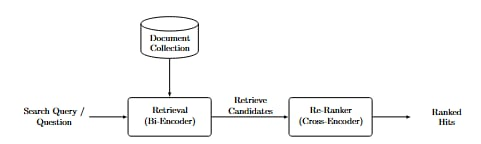
\includegraphics[width=1\textwidth]{images/retrieval.jpg}
    \caption{Sơ đồ quy trình truy xuất hai giai đoạn (Retrieval \& Re-ranking)}
    
\end{figure}
   
    
    % --- 2. PHẦN HIỆN THỰC (IMPLEMENTATION) ---
    \subsubsection{Chi tiết hiện thực kỹ thuật}
    Hệ thống được hiện thực hóa bằng thư viện \texttt{sentence-transformers} và \texttt{qdrant-client}, trải qua 4 bước xử lý tuần tự:
    
    \paragraph{Bước 1: Tìm kiếm Vector (Candidate Generation):}
    Mục tiêu là thu hẹp không gian tìm kiếm từ toàn bộ cơ sở dữ liệu xuống một tập ứng viên nhỏ.
    \begin{itemize}
        \item \textbf{Mã hóa:} Câu truy vấn được vector hóa và chuẩn hóa (\texttt{normalize\_embeddings=True}) để tương thích với độ đo Cosine.
        \item \textbf{Truy vấn Qdrant:} Hệ thống thực hiện \texttt{query\_points} với tham số giới hạn \texttt{limit=30}. Ngưỡng 30 này đóng vai trò là "Bộ lọc thô", đủ rộng để bao quát các ngữ cảnh tiềm năng.
        \item \textbf{Payload:} Dữ liệu trả về bao gồm cả văn bản gốc (\texttt{text\_original}) để phục vụ bước tiếp theo.
    \end{itemize}
    \begin{lstlisting}[language=Python,  label={lst:retrieval_logic}]
            query_vec = embed_model.encode([query], normalize_embeddings=True)[0].tolist()
            resp = self.client.query_points(
                    collection_name=self.collection_name,
                    query=query_vec,                 
                    # query_filter=query_filter,     
                    limit=30,
                    with_payload=True
                )
    
            hits = resp.points or []
            
            
            if not hits: return []
    \end{lstlisting}
    
    \paragraph{Bước 2: Đánh giá ngữ nghĩa chéo (Cross-Encoder Scoring):}
    Đây là bước tinh lọc quan trọng nhất. Hệ thống sử dụng mô hình \texttt{BAAI/bge-reranker-large} — một mô hình SOTA (State-of-the-art) về khả năng rerank đa ngôn ngữ.
    \begin{itemize}
        \item Hệ thống ghép cặp \texttt{(Câu hỏi, Đoạn văn bản)} từ 30 ứng viên ở Bước 1.
        \item Danh sách các cặp \texttt{[Query, Document]} này sau đó được đưa vào mô hình để thực hiện dự đoán song song (\texttt{prediction}), tạo ra điểm số tương đồng ngữ nghĩa chính xác cho từng ứng viên.
    \end{itemize}
    \begin{lstlisting}[language=Python,  label={lst:retrieval_logic}]
     # 2. Rerank
            pairs = []
            for hit in hits:
                if hit.payload:
                    pairs.append([query, hit.payload.get('text_original', '')])
            
            if not pairs: return []
    
            scores = rerank_model.predict(pairs) # type: ignore
    \end{lstlisting}
    \paragraph{Bước 3: Chọn lọc kết quả (Final Selection):}
    Dựa trên điểm số mới từ Cross-Encoder, danh sách được sắp xếp lại (\texttt{sorted}) theo thứ tự giảm dần.
    \begin{itemize}
        \item Hệ thống thực hiện cắt ngưỡng lấy \textbf{Top-5} kết quả tốt nhất (\texttt{[:5]}).
        \item \textbf{Ý nghĩa:} Con số 5 được lựa chọn thực nghiệm nhằm tối ưu hóa bộ nhớ đệm (Context Window) của LLM, đảm bảo mô hình chỉ nhận được những thông tin tinh túy nhất, giảm thiểu hiện tượng ảo giác do nhiễu thông tin.
    \end{itemize}
    \begin{lstlisting}[language=Python,  label={lst:retrieval_logic}]
     # Top 5
            ranked_hits = sorted(zip(scores, hits), key=lambda x: x[0], reverse=True)[:5]
    \end{lstlisting}
    \paragraph{Bước 4: Mở rộng ngữ cảnh (Context Augmentation):}
    Một thách thức đặc thù của dữ liệu hội thoại là tính liên kết ngữ nghĩa giữa các lượt lời. Một câu nói đơn lẻ (ví dụ: \textit{"Tôi đồng ý với ý kiến đó"}) sẽ trở nên vô nghĩa nếu thiếu câu nói trước đó. Để giải quyết vấn đề này, hệ thống áp dụng kỹ thuật \textbf{Cửa sổ trượt (Sliding Window)} để mở rộng ngữ cảnh xung quanh kết quả tìm kiếm.
    
    Dựa trên chỉ số (\textit{index}) của đoạn hội thoại tìm được trong chuỗi thời gian gốc, hệ thống thực hiện truy xuất thêm các đoạn lân cận:
    \begin{itemize}
        \item \textbf{Cơ chế:} Với mỗi kết quả $h_i$ tại vị trí $k$, hệ thống sẽ lấy thêm đoạn $k-1$ (lượt lời trước đó) và $k+1$ (lượt lời sau đó).
        \item \textbf{Mục đích:} Việc lấy thêm đoạn $k-1$ giúp giải quyết các tham chiếu đại từ (như "đó", "anh ấy"), trong khi đoạn $k+1$ cung cấp phản hồi ngay lập tức.
        \item \textbf{Hợp nhất \& Khử trùng:} Hệ thống sử dụng một tập hợp \texttt{processed\_ids} để đảm bảo các đoạn hội thoại không bị lặp lại nếu các kết quả tìm kiếm nằm quá gần nhau.
    \end{itemize}
    \begin{lstlisting}[language=Python,  label={lst:retrieval_logic}]
    # 3. Context Augmentation 
            final_chunks = []
            processed_ids = set()
            
            # Map ID to index 
            id_to_index = {uid: i for i, uid in enumerate(self.kb_memory["utterance_order"])}
            
            for score, hit in ranked_hits:
                if not hit.payload: continue
                doc_id = hit.payload.get('doc_id')
                if not doc_id or doc_id in processed_ids: continue
                
                idx = id_to_index.get(doc_id)
                if idx is None: continue
                
                # Window [idx-1, idx+1]
                start = max(0, idx - 1)
                end = min(len(self.kb_memory["utterance_order"]), idx + 2)
                
                chunk_text = []
                for i in range(start, end):
                    uid = self.kb_memory["utterance_order"][i]
                    processed_ids.add(uid)
                    u = self.kb_memory["utterances"][uid]
                    chunk_text.append(f"[{u['start']}] {u['speaker']}: {u['text']}")
                
                final_chunks.append("\n".join(chunk_text))
                
            return final_chunks
    \end{lstlisting}